\chapter{The Global Signal -- Its Physics and Significance to Cosmology}

\section{Overview of the Epoch of Reionization}

In brief, the Epoch of Reionization refers to the period of the universe's 
history during which its supply of intergalactic hydrogen became reionized.  
This is important to its evolution, and therefore of interest to astronomers, 
due to the driving factor of that ionization: the ignition of the first stars, 
galaxies, and black holes in the universe. A positive detection of the Epoch of 
Reionization will help astronomers to clarify many open questions of cosmology, 
such as the properties of the first galaxies, how stars with zero metallicity 
formed, the physics of early quasars, and more.

In slightly more detail, let us begin at the beginning. At the start of time, 
the universe was extremely hot and ionized from the Big Bang. Over time, as 
space itself expanded and the gas within the universe cooled adiabatically 
along with that expansion, the temperature of the universe dropped low enough 
that the nearly uniform ionized plasma that made up the universe was able to 
recombine to form neutral hydrogen. This phase transition, which occurred 
approximately 400,000 years after the Big Bang, enabled photons to decouple 
from the baryonic matter, allowing photons to stream freely for the first time 
in the history of the universe.  Those photons are what we now know as the 
``Cosmic Microwave Background" (CMB).

At the point of the CMB, the gravitational force had heretofore always served 
as second fiddle to the electromagnetic force, and the formation of structure 
was driven solely by dark matter~\citep{zaroubi2012}.  As such, structure had 
yet to form, and the release of the CMB led to a period known as the ``Dark 
Ages" -- a time when the universe had nothing to do but slowly get to work 
allowing slight matter over-densities grow and transform into stars, galaxies, 
and black holes.

So, about 100 million years passed and the universe bathed in nothing but the 
after-glow of the Big Bang. Finally, the first galaxies formed, and along with 
them bright stars to emit ionizing radiation. Soon, we find small ionized 
bubbles in the intergalactic medium (IGM), the hydrogen gas filling the space 
between galaxies. Over time, more galaxies and their bright stars make more 
ionized bubbles, until eventually the entire universe's supply of loose 
hydrogen gas has been converted into a proton-electron ionized plasma.

This period, very creatively, is called the Epoch of Reionization -- the epoch 
during which the universe once again became ionized, like it was at the dawn of 
time.

As of yet, there has been no confirmed direct detection of this time period -- 
either of the objects that drive it nor of the gas behavior itself. This is not 
for lack of trying. There are currently (or soon to be) observatories looking 
for high-redshift galaxies and quasars~\citep{gardner2006}, for power-spectrum 
measurements to find ionized regions around those high-energy 
objects~\citep{deboer2017}, and for the microscopic temperature changes in the 
gas of the universe~\citep{bowman2018}.  As it turns out, these observations 
are hard to make -- 13 billion light years is a long way for light to travel.

For the sake of brevity and intellectual focus, this thesis (and the experiment 
proposed within) will be focusing solely on observing the overall average 
behavior of the intergalactic medium as it evolves throughout this time period.  
This is referred to as the ``global signal".

\section{Overview of the Global Signal}

The global signal of reionization is an observation of the overall average 
nature of hydrogen throughout this epoch, i.e. the spatially averaged signal 
from the neutral hydrogen gas, as observed using redshifted 21 cm emission from 
the intergalactic medium 13 billion years ago. More specifically, global signal 
experiments seek to observe the relationship between the gas temperature and 
the ambient temperature of the universe, as set by the CMB photons.  By 
observing the evolution of the thermal gas temperature ($T_K$) relative to the 
photon temperature ($T_\gamma$), we are able to better understand how and when 
energy was injected into the gas~\citep{pritchard-loeb2010}. For example, the 
X-rays generated by black holes contributed to the heating of the gas, making 
the gas itself brighter than the ambient photons. Additionally, Lyman-$\alpha$ 
photons from Population II and III stars modify the coupling of the IGM gas 
temperature to the 21 cm spin temperature via the Wouthuysen-Field effect, 
providing a means to track early star formation~\citep{furlanetto2006}.

This signal ($T_b$) is measured as a function of four main variables -- the 
thermal temperature of the hydrogen gas ($T_K$), the volume-averaged ionized 
fraction of hydrogen ($x_i$), the specific flux of the Lyman-$\alpha$ frequency 
($J_\alpha$), and the number density of hydrogen ($n_H$). One particularly 
convenient aspect of $T_b$ is that its dependence on each of these quantities 
saturates at some point, leading to clear and separate regimes in the history 
of the signal that can only be described by the changes in one 
variable~\citep{pritchard-loeb2012}. These regimes can be seen in 
Fig.~\ref{fig:global-signal}, and are physically detailed below.

\begin{figure}
    \begin{center}
    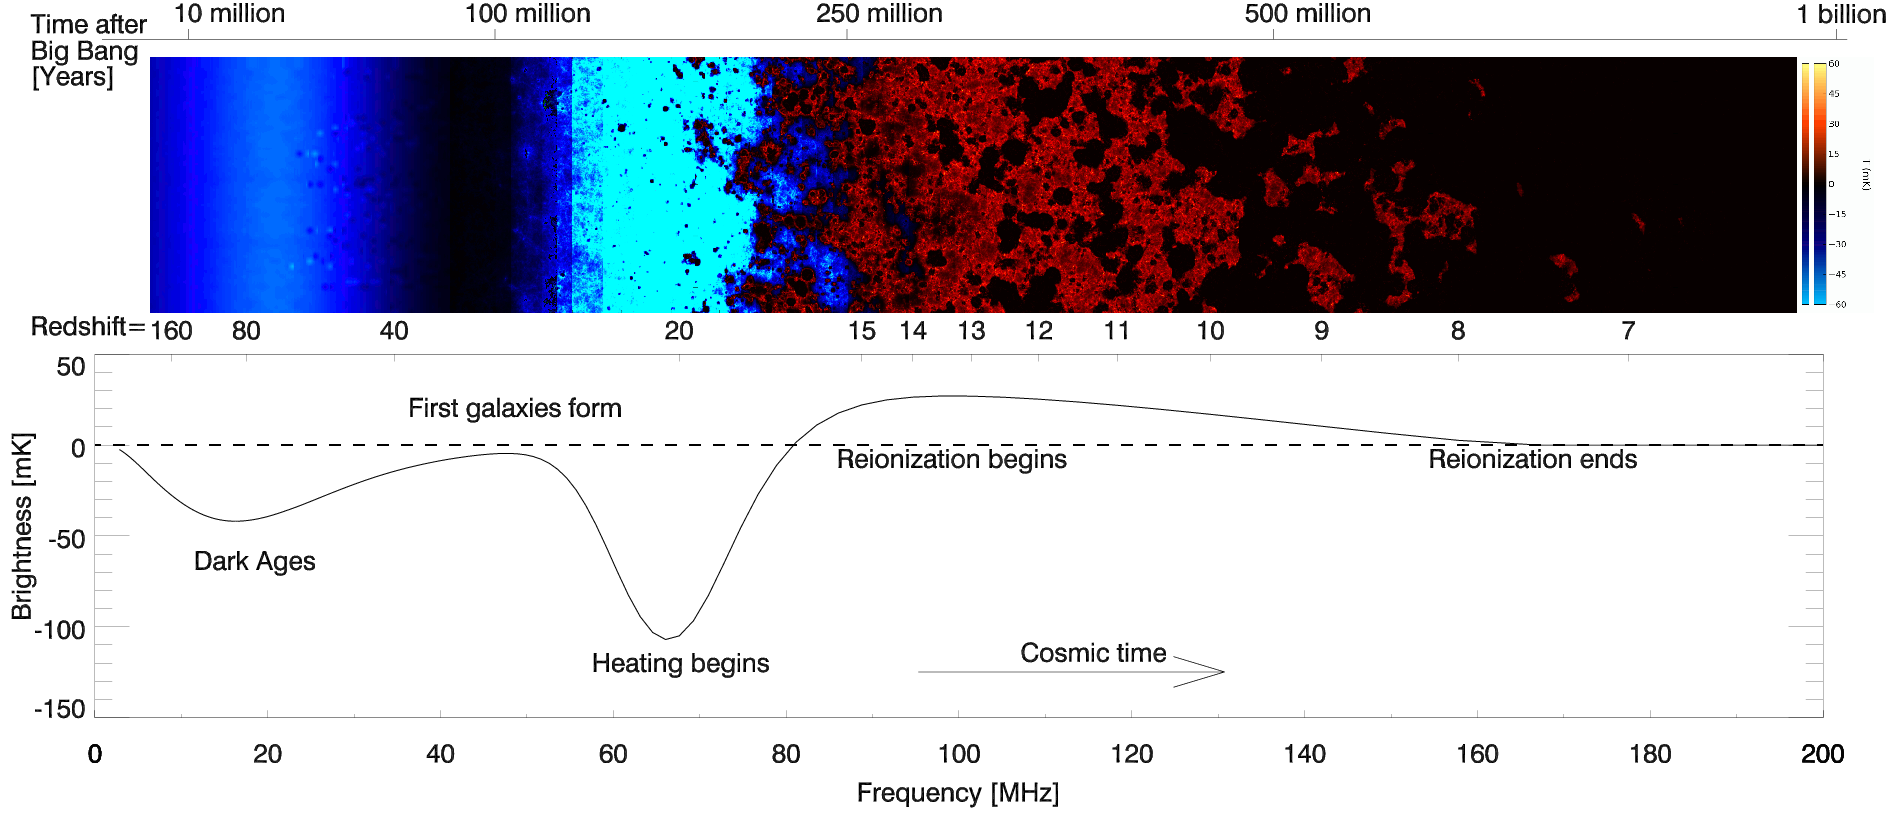
\includegraphics[width=\linewidth]{global_signal.png}
    \end{center}
    \caption{
        In the top half of the figure, we see a cartoon of the reionization 
        history of the universe and the development and growth of ionized 
        bubbles over time. In the bottom half, we see a breakdown of $T_b$, the 
        brightness temperature of the 21 cm global signal, over time. There are 
        five labeled regimes to this plot, each corresponding to the dominance 
        of a different variable in the production of the 21 cm signal. Figure 
        originally published in~\citealp{pritchard-loeb2012}.
    }
    \label{fig:global-signal}
\end{figure}

\subsection{Brief History of the Global Signal}
\begin{itemize}
    \item[--] (200 $\leq z \leq$ 1100): During this time period, the residual 
     free electron fraction remaining post-recombination and the high gas 
     density allows the thermal and spin temperatures of the gas to remain 
     coupled with the photon background via Compton scatting and collisional 
     excitations. All temperatures are the same, and therefore there will be no 
     detectable 21 cm signal.
    \item[--] (40 $\leq z \leq$ 200): As cosmological expansion continues, 
     Compton scattering no longer couples the thermal temperature of the gas to 
     the CMB photons, and the gas and radiation decouple and go out of 
     equilibrium.  Collisional coupling sets the spin temperature $T_S < 
     T_\gamma$, leading to an absorption feature in the 21 cm global signal.  
    \item[--] (30 $\leq z \leq$ 40): Expansion continues and collisional 
     interactions are no longer effective at coupling the thermal and spin 
     temperatures of the gas. The excitation levels shift to being set by 
     radiative coupling to the CMB, such that $T_S = T_\gamma$, and there is no 
     detectable 21 cm signal.
    \item[--] (15 $\leq z \leq$ 30): As the first sources (e.g. stars, active 
     galactic nuclei (AGN), etc...) ignite, they begin emitting high energy 
     Lyman-$\alpha$ and X-ray photons. The hyperfine populations couple to the 
     thermal temperature of the cold gas via the Wouthuysen-Field effect, such 
     that $T_S \sim T_K < T_\gamma$, resulting in an absorption feature in the 
     21 cm global signal.
    \item[--] (7 $\leq z \leq$ 15): The radiation (particularly the X-rays) 
     from bright sources heat the gas, $T_K > T_\gamma$ and we see 21 cm 
     emission in the global signal. Lyman-$\alpha$ coupling is still effective 
     at setting the level populations.
    \item[--] ($z \leq$ 7): Enough ionizing radiation has spread throughout the 
     universe that the IGM has been converted from neutral to ionized, and 
     reionization is complete.
\end{itemize}

